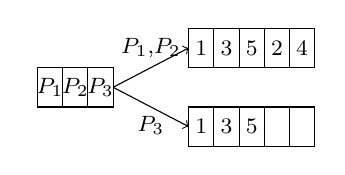
\begin{tikzpicture}[font=\footnotesize]
    % Define the width and height of the rectangles
    \def\rectwidth{0.32}
    \def\rectheight{0.5}
    \def\listdist{1.6}
        
    % Draw the queue
    \draw (-\rectwidth,0) rectangle (\rectwidth,\rectheight);
    \node at (-\rectwidth/2,\rectheight/2) {$P_1$};

    \draw (0,0) rectangle (\rectwidth,\rectheight);
    \node at (\rectwidth/2,\rectheight/2) {$P_2$};

    \draw (\rectwidth,0) rectangle (2*\rectwidth,\rectheight);
    \node at (\rectwidth+\rectwidth/2,\rectheight/2) {$P_3$};
%     
    % Add arrows from the head of the queue
    \draw[->] (2*\rectwidth,\rectheight/2) -- (\listdist,3*\rectheight/2) node[midway, above] {$P_1$,$P_2$};
    \draw[->] (2*\rectwidth,\rectheight/2) -- (\listdist,-\rectheight/2) node[midway, below] {$P_3$};
  
    \foreach \x in {0,1,2,3,4} {
      \draw (\listdist+\x*\rectwidth,\rectheight) rectangle (\listdist+\x*\rectwidth+\rectwidth,2*\rectheight);
      \draw (\listdist+\x*\rectwidth,-\rectheight) rectangle (\listdist+\x*\rectwidth+\rectwidth,0);
    }

    \node at (\listdist+\rectwidth/2,-\rectheight/2) {1};
    \node at (\listdist+\rectwidth+\rectwidth/2,-\rectheight/2) {3};
    \node at (\listdist+2*\rectwidth+\rectwidth/2,-\rectheight/2) {5};

    \node at (\listdist+\rectwidth/2,3*\rectheight/2) {1};
    \node at (\listdist+\rectwidth+\rectwidth/2,3*\rectheight/2) {3};
    \node at (\listdist+2*\rectwidth+\rectwidth/2,3*\rectheight/2) {5};
    \node at (\listdist+3*\rectwidth+\rectwidth/2,3*\rectheight/2) {2};
    \node at (\listdist+4*\rectwidth+\rectwidth/2,3*\rectheight/2) {4};
\end{tikzpicture}

%%% Local Variables:
%%% mode: latex
%%% TeX-master: "../distributed_mrf"
%%% End:
